% section4_diagnostics.tex — Module C: Zhe
\section{Sampler Behaviour and Convergence Diagnostics}\label{sec:diagnostics}

Prior to model fitting, all variables were z-score standardised:
predictors \texttt{temp} and \texttt{hum} and the response \texttt{cnt}
were each transformed to zero mean and unit variance, so that the
regression coefficients $\beta_j$ are of order unity and the weakly
informative prior $\mathcal{N}(0, 10^2)$ is genuinely diffuse relative
to the posterior scale.

The model was fitted using PyMC with the No-U-Turn Sampler (NUTS),
running 4 independent chains of 2{,}000 post-warmup draws each
(8{,}000 total), preceded by 1{,}000 tuning steps that were discarded
prior to inference.

\subsection{Trace Plots}

Visual inspection of the trace plots (Figure~\ref{fig:trace}) reveals
that all four chains for $\beta_0$, $\beta_1$, $\beta_2$, and $\sigma$
exhibit the characteristic ``hairy caterpillar'' appearance: sample
paths fluctuate around stable means with no visible upward or downward
drift, and the four chains overlap substantially throughout the entire
post-warmup period. This confirms both \emph{stationarity} (the chain
has reached its stationary distribution) and \emph{good mixing} (the
sampler explores the posterior efficiently without becoming trapped in
local regions). The posterior KDE plots confirm unimodal, approximately
symmetric distributions for all parameters.

\begin{figure}[htbp]
    \centering
    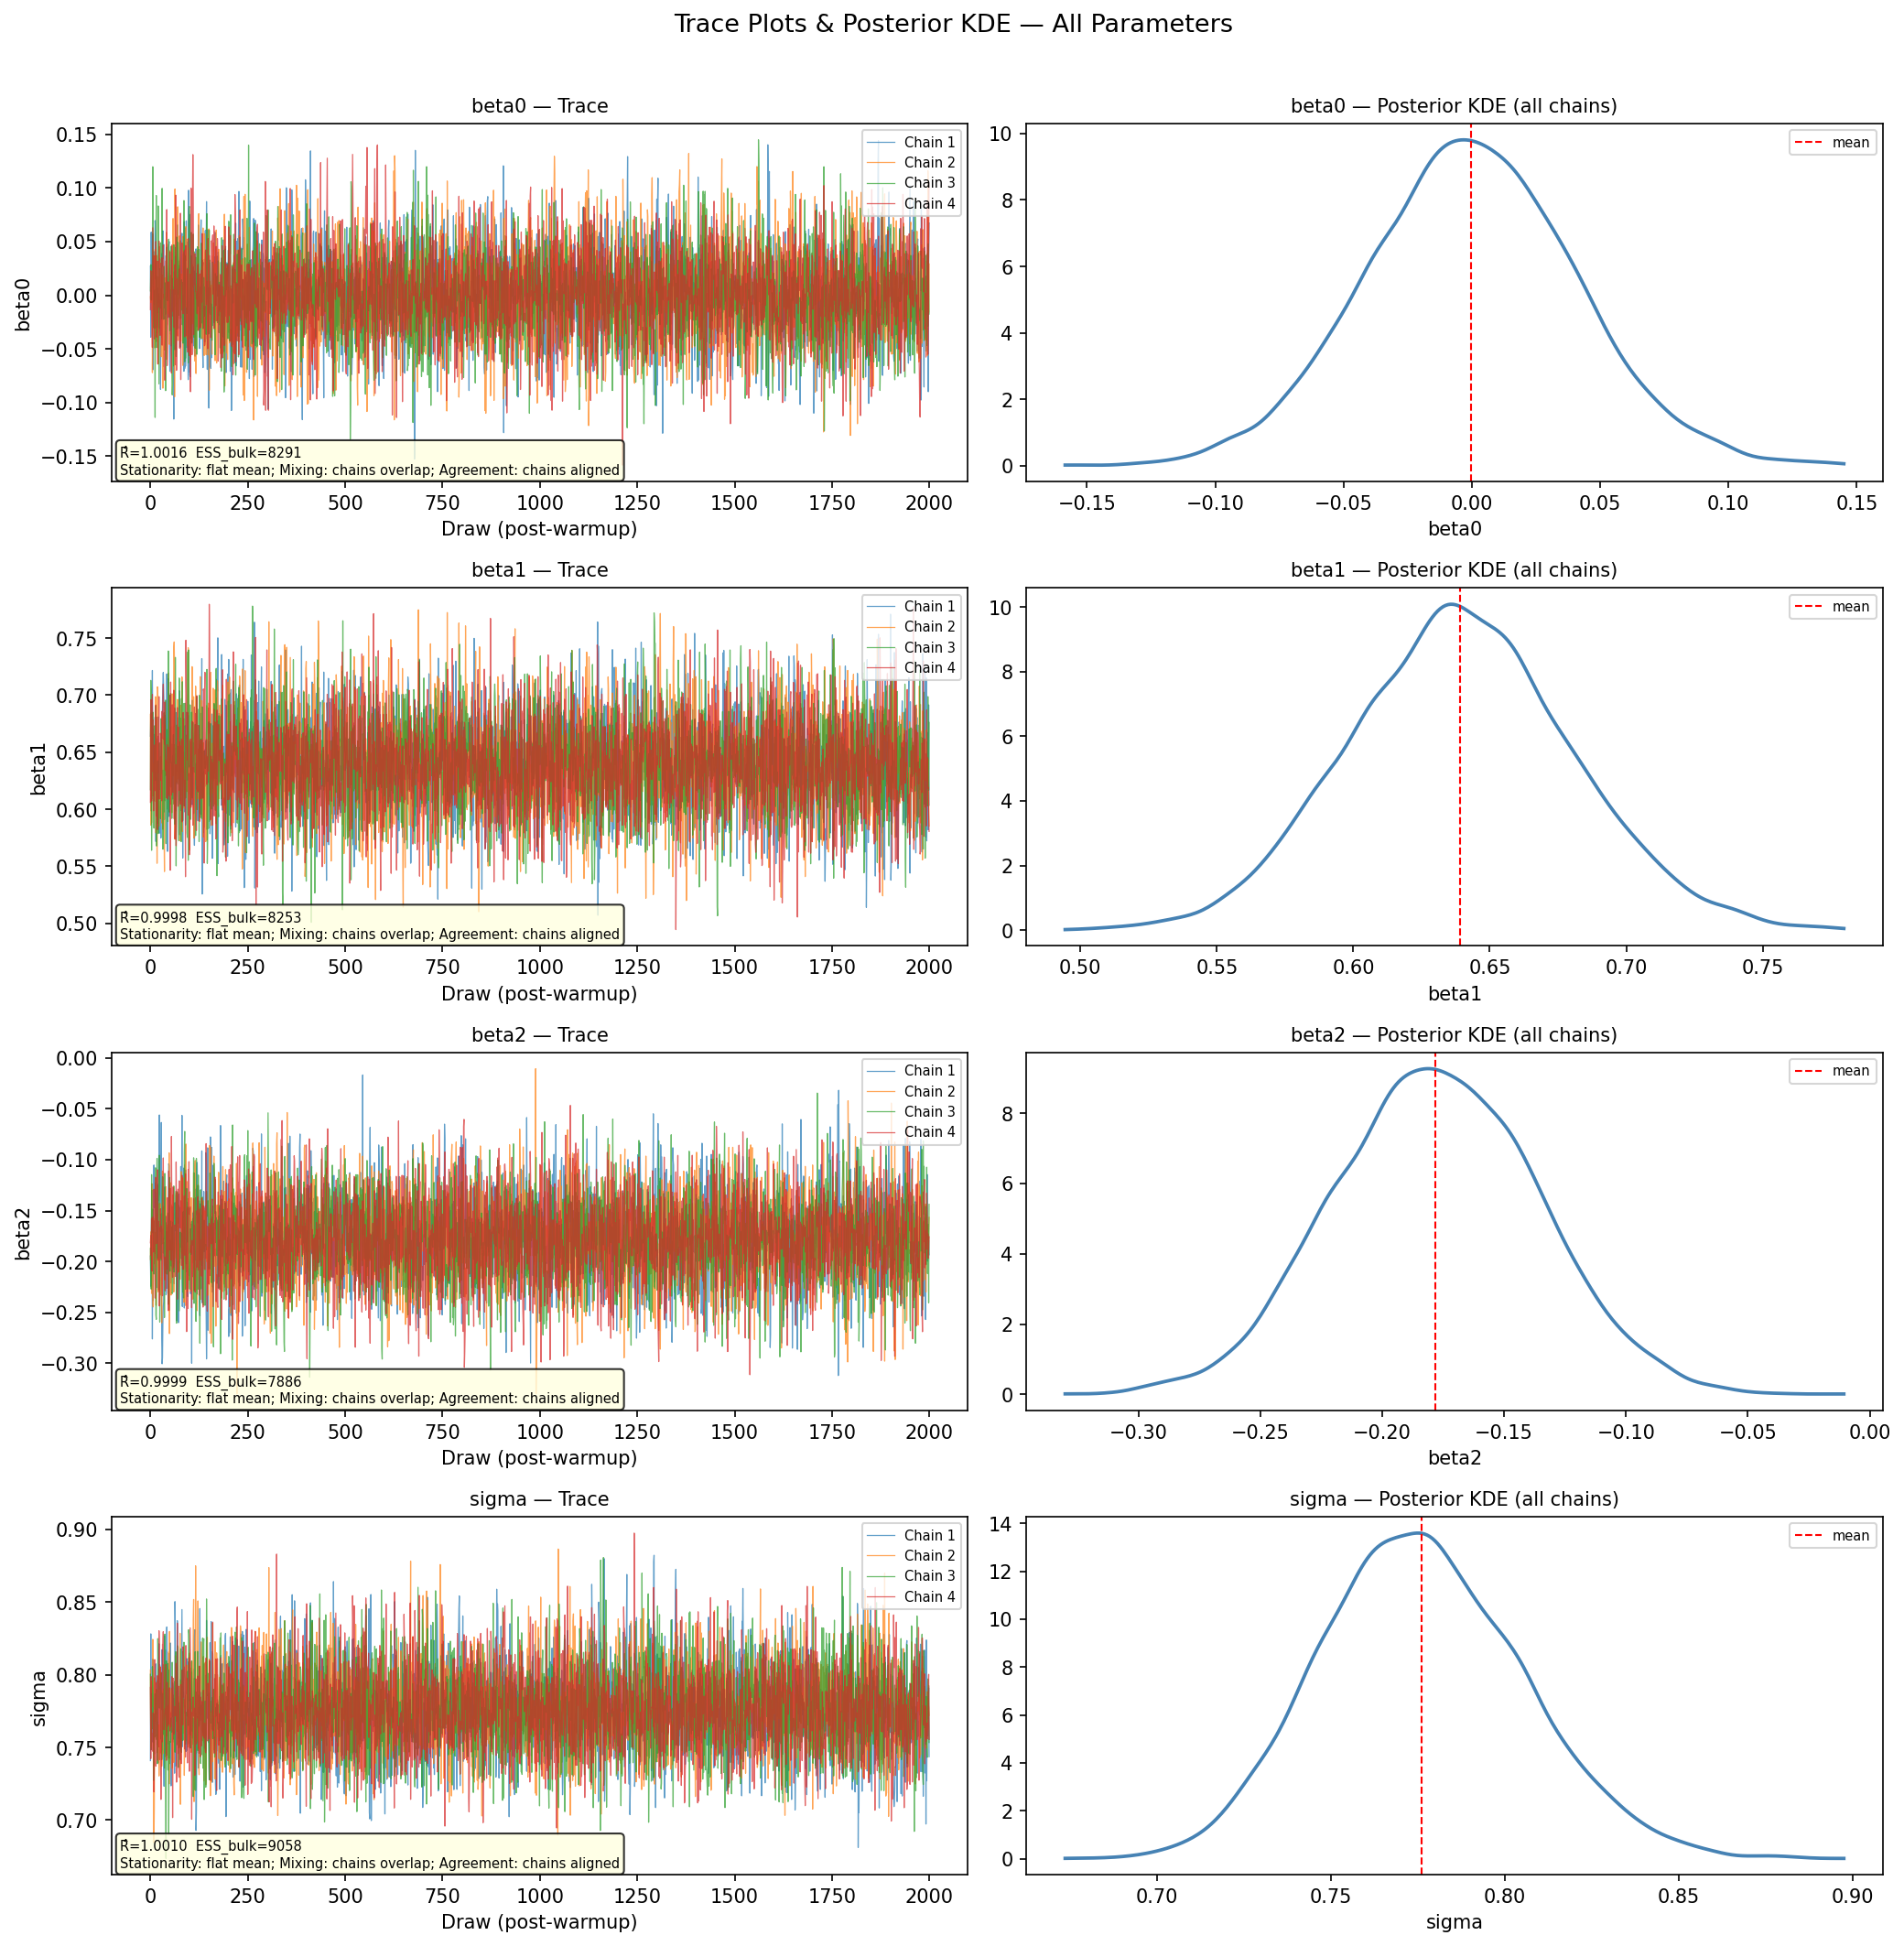
\includegraphics[width=\textwidth]{../results/figures/trace_plots.png}
    \caption{Trace plots and posterior KDE for all parameters. All chains
    show stable, overlapping trajectories consistent with convergence.}
    \label{fig:trace}
\end{figure}

\subsection{Gelman--Rubin Statistic ($\hat{R}$)}

The $\hat{R}$ statistic compares between-chain variance to within-chain
variance; values close to 1.0 indicate that all chains have converged
to the same distribution \citep{gelman1992inference}. All parameters
yielded $\hat{R} < 1.01$: specifically,
$\hat{R}(\beta_0) = 1.002$,
$\hat{R}(\beta_1) = 1.000$,
$\hat{R}(\beta_2) = 1.000$, and
$\hat{R}(\sigma)  = 1.001$,
confirming satisfactory convergence across all chains.

\subsection{Effective Sample Size}

The bulk and tail effective sample sizes (ESS) quantify the number of
effectively independent draws after accounting for within-chain
autocorrelation. All parameters achieved $\text{ESS}_{\text{bulk}} >
7{,}800$ (range: 8{,}253--9{,}058) and $\text{ESS}_{\text{tail}} >
5{,}100$, far exceeding the recommended threshold of
$\max(400,\; 0.1 \times N_{\text{total}}) = 800$ for 8{,}000 total
draws. The autocorrelation plots (Figure~\ref{fig:autocorr}) confirm
rapid decay to zero within the first 5--10 lags, consistent with
efficient NUTS sampling.

\begin{figure}[htbp]
    \centering
    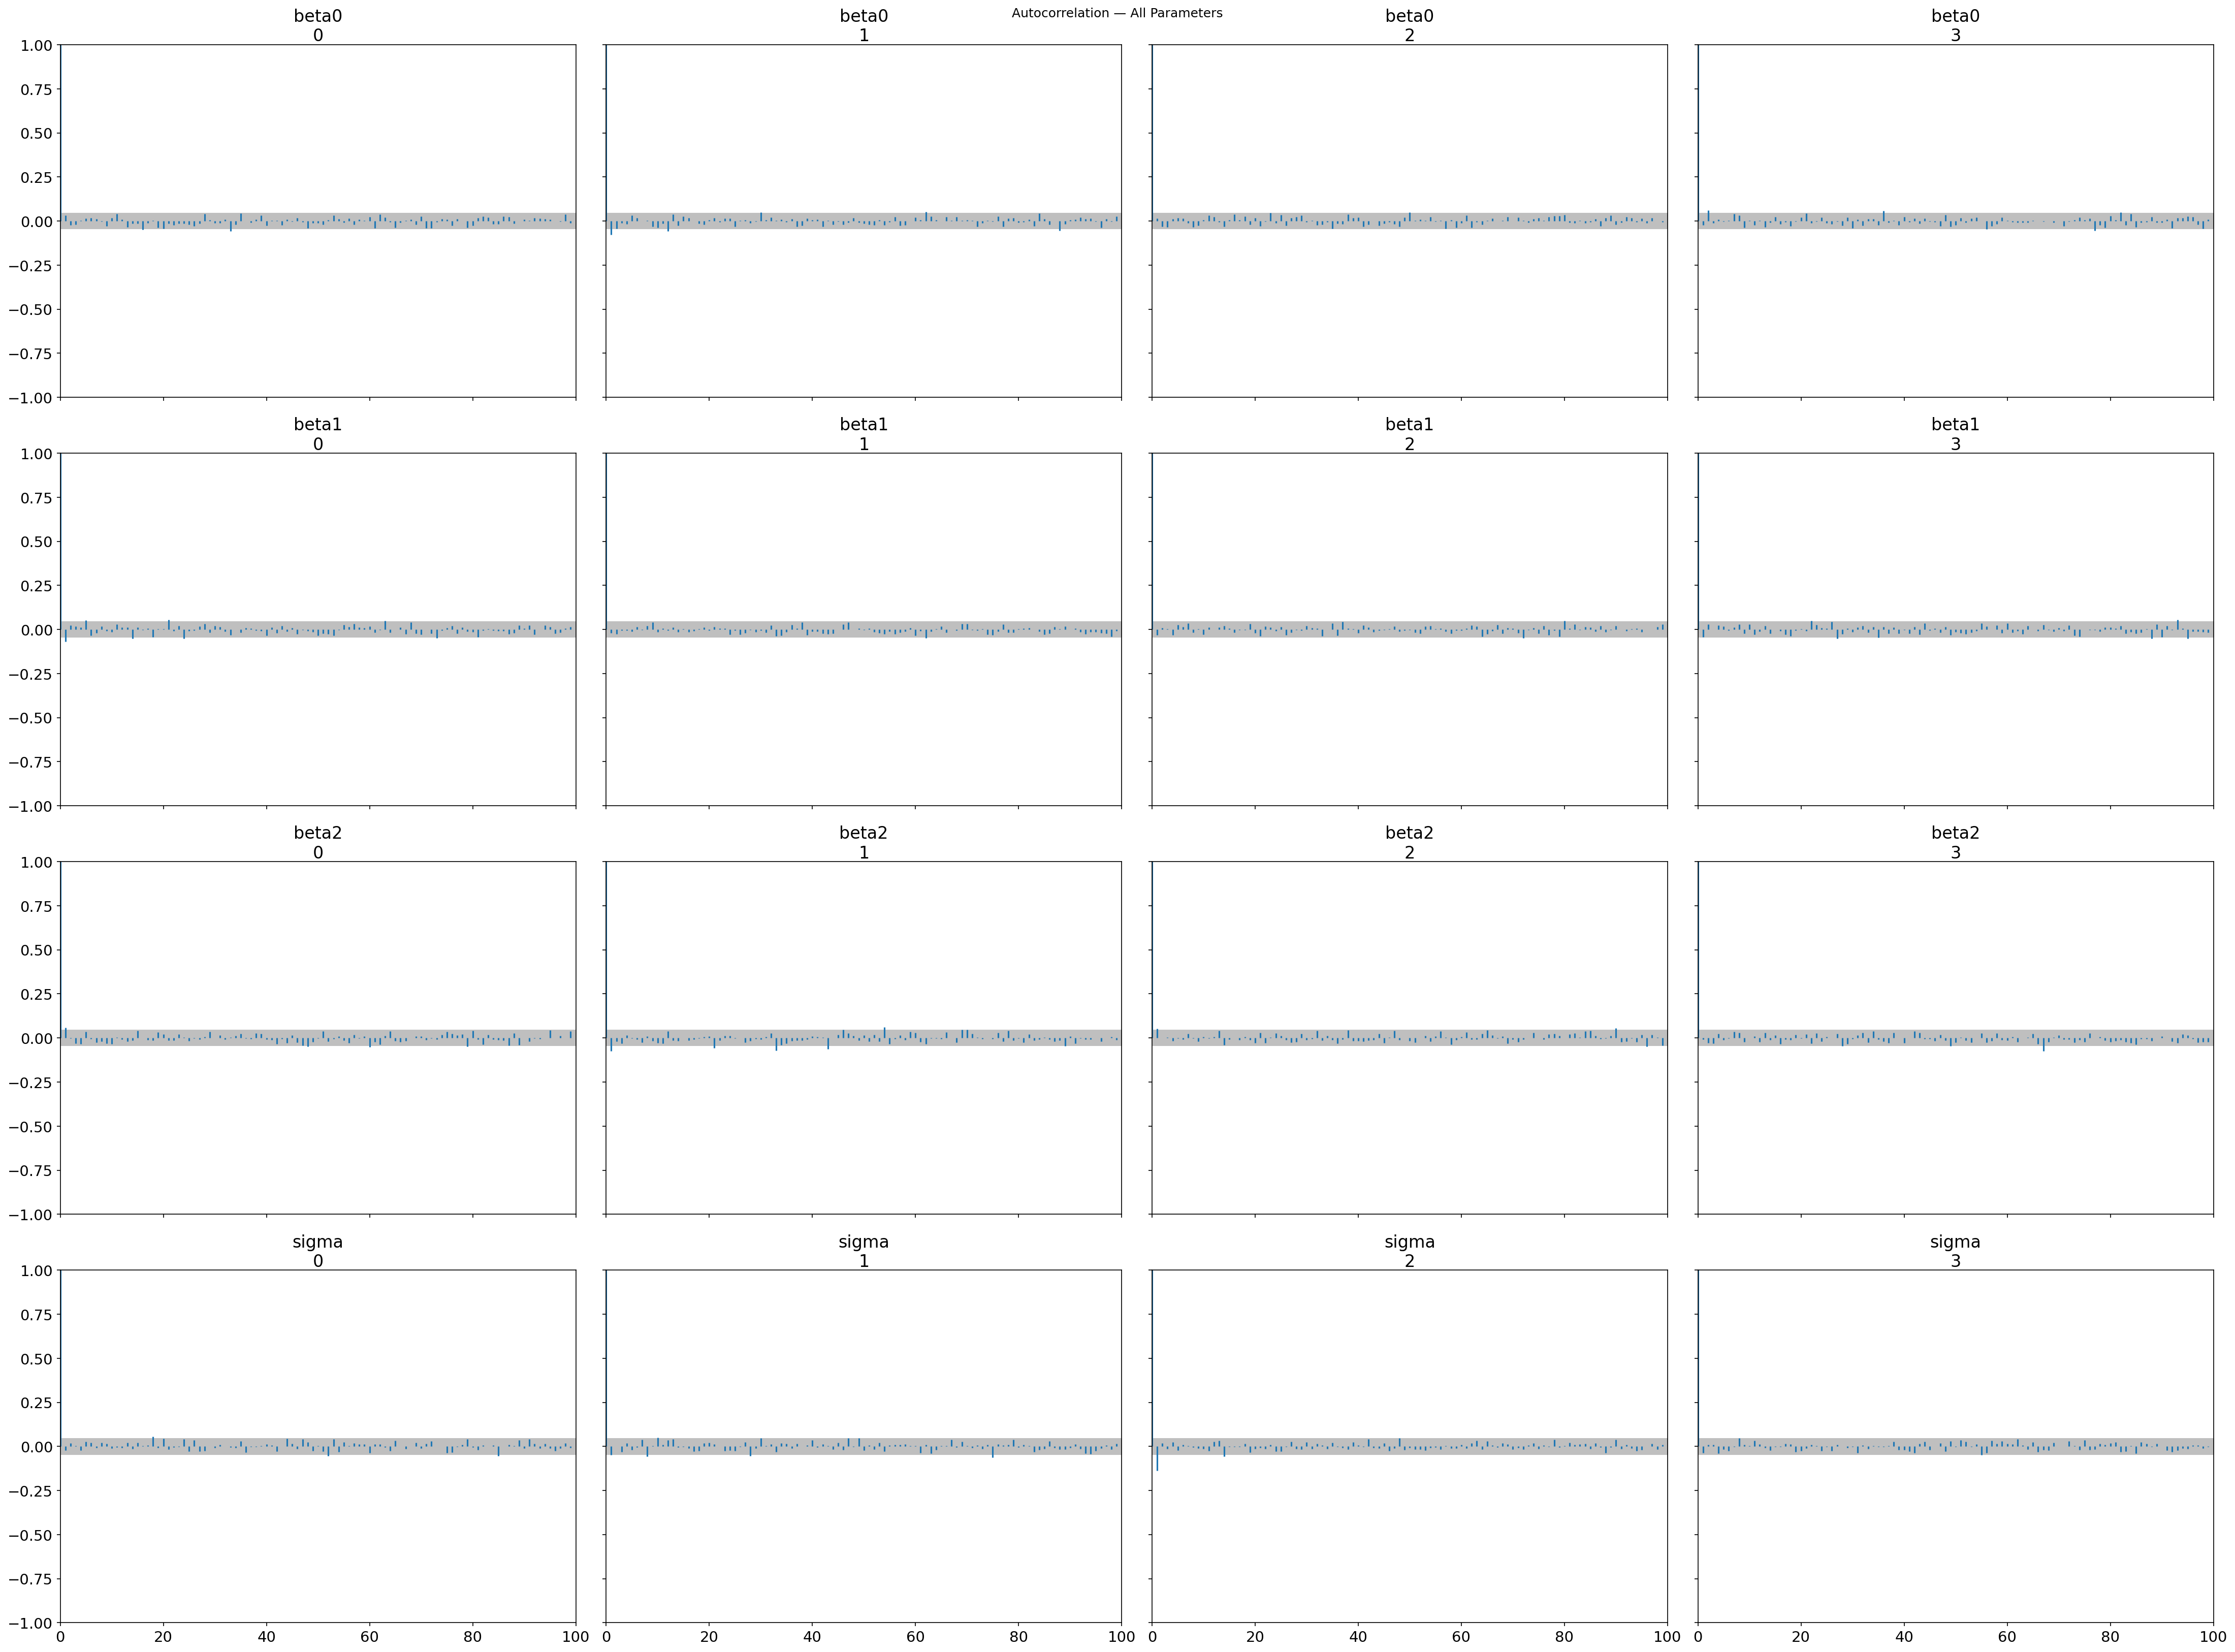
\includegraphics[width=\textwidth]{../results/figures/autocorr.png}
    \caption{Autocorrelation plots for all parameters. Autocorrelation
    decays to zero within 5--10 lags, indicating low within-chain
    dependence and high effective sample size.}
    \label{fig:autocorr}
\end{figure}

\subsection{Burn-in Justification}

The 1{,}000 tuning draws per chain were discarded as burn-in. This
decision is justified on two grounds. First, the trace plots show that
all chains reach their stationary regions within the first 100--200
post-warmup draws, indicating that 1{,}000 tuning steps were more than
sufficient. Second, the $\hat{R} < 1.002$ and
$\text{ESS}_{\text{bulk}} > 7{,}800$ values jointly confirm that the
retained draws constitute a reliable, low-autocorrelation posterior
sample. No divergent transitions were recorded (0 out of 8{,}000
draws), providing additional evidence that the sampler explored the
posterior geometry without difficulty.

\begin{table}[htbp]
    \centering
    \caption{Posterior summary statistics for all parameters.}
    \label{tab:summary}
    \begin{tabular}{lrrrrrr}
        \hline
        Parameter & Mean & SD & 95\% HDI (low) & 95\% HDI (high) & $\hat{R}$ & ESS$_\text{bulk}$ \\
        \hline
        $\beta_0$ & $-0.001$ & $0.041$ & $-0.080$ & $0.075$ & $1.002$ & $8{,}291$ \\
        $\beta_1$ & $0.639$  & $0.041$ & $0.562$  & $0.716$ & $1.000$ & $8{,}253$ \\
        $\beta_2$ & $-0.178$ & $0.042$ & $-0.253$ & $-0.096$ & $1.000$ & $7{,}886$ \\
        $\sigma$  & $0.776$  & $0.029$ & $0.724$  & $0.833$ & $1.001$ & $9{,}058$ \\
        \hline
    \end{tabular}
\end{table}
